\section{Main ellipse and Animation Controls}
\label{sec:09-ellipse-anim}

Before a particular triangle family can be setup and its loci visualized, one must set certain basic animation controls, using the various areas highlighted in \cref{fig:09-animation}. These include (i) the setting of the base ellipse aspect ratio \texttt{a/b} either via typing into the textbox (showing $1.618$ in the picture) or via the scrollbar next to it; (ii) above the animation area, pausing or running the animation and choosing a speed -- slow, medium, or fast. Note: a small ``anim'' dropbox located below the \texttt{a/b} scrollbar, when not in the ``off'' position, triggers a smooth oscillation of the aspect ratio over the range specified in the ``min'' and ``max'' input boxes to its right.

\begin{figure}
    \centering
    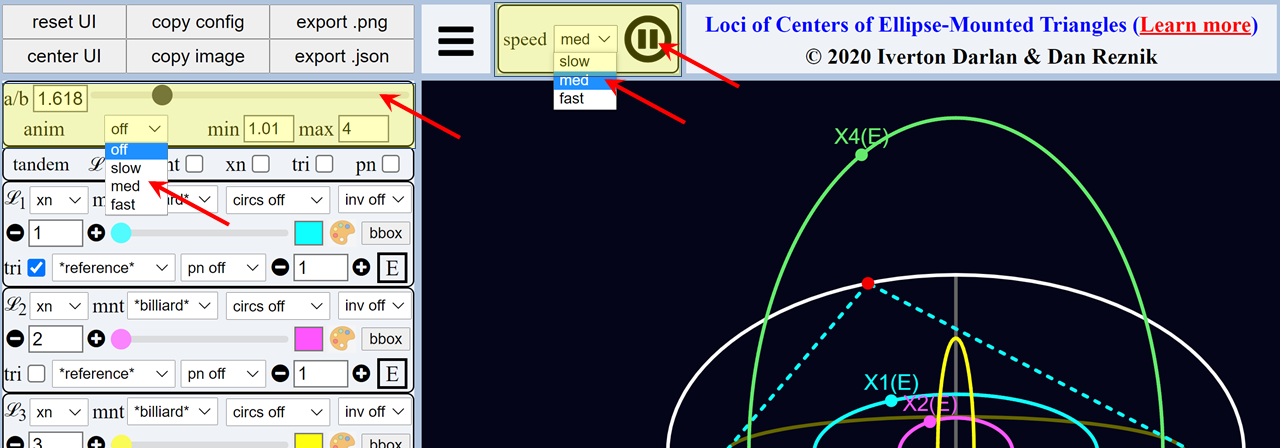
\includegraphics[width=\textwidth]{pics_09_130_animation.png}
    \caption{Basic animation controls include (i) the setting of the base ellipse aspect ratio \texttt{a/b} either via typing into the textbox (showing $1.618$ in the picture) or via the scrollbar next to it; (ii) above the animation area, pausing or running the animation and choosing a speed -- slow, medium, or fast. Note: a small ``anim'' dropbox located below the \texttt{a/b} scrollbar, when not in the ``off'' position, triggers a smooth oscillation of the aspect ratio over the range specified in the ``min'' and ``max'' input boxes to its right.}
    \label{fig:09-animation}
\end{figure}

\subsection{Convenience Animation Controls}

If the animation is paused, hitting the up (or right) and down (or left) arrows on the keyboard allows one to carefully step forward or backward over the triangle family.

The mouse wheel allows for the simulation image to be zoomed or unzoomed.

By clicking and dragging into the main animation area one can pan and reposition the image.